\documentclass[letter]{article}

\usepackage{amsmath}
\usepackage{graphicx}
\usepackage{geometry}
\usepackage{braket}
\usepackage{framed}
\usepackage{fancyhdr}
\geometry{
  letterpaper,
  left=1in,
  right=1in,
  bottom=1in,
  top=1in}
\pagestyle{fancy}
\lhead{NE101 Midterm 2 Study Guide}
\chead{}
\rhead{\sectionmark}
\lfoot{}
\cfoot{\thepage}
\rfoot{}
\setlength\parindent{0pt}

\begin{document}
\textbf{\Large{Nuclear Engineering 101: Midterm 2 Study Guide}} \\
Joshua Rehak
\vspace{12pt}
%\cite[pp. 45]{krane}
%\cite[Lec 24]{lecture}

\textbf{Note:} Everything in this guide is from the text (Krane) or
lecture, or office hours. I have tried my best to cite everything as
completely as possible, but some of the info may be from office
hours. I didn't think of any of this on my own.

\section{Nuclear Electromagnetic Moments}

Ref: \cite[pp. 71-75]{krane},\cite[Lec 10]{lecture}

A distribution of electric charge and/or current will create an
electric potential. This can be described by the ``multipole
moment''. \\

Note the values of $L$ are the \textit{order of the moment}, not
angular momentum.

\subsection{Electric multipoles}

\begin{itemize}
\item Monopole moment: $L=0$, this is just the spherical nucleus, the electric
  potential looks like $V = \frac{Q}{R}$. 
\item Dipole moment: $L=1$. The electric dipole is just linear
  translation of the nucleus. $V=0$, see below.
\item Quadrupole moment: $L=2$, the electric potential is from the
  nucleus squishing in one direction and then the other. The amount of
  quadrupole moment can be calculated:
  \begin{equation*}
    eQ=e\int\psi^*(3z^2-r^2)\psi~d^3\vec{r}
  \end{equation*}
  If the nucleus is spherical,
  $\braket{z}^2=\braket{x}^2=\braket{y}^2$, so $eQ=0$. The higher the
  value of $eQ$ the more deformed the nucleus is.
\end{itemize}

All electric moments have parity determined by $(-1)^L$. If you want
to do some kind of electromagnetic operation on a state ($\psi$) with
some operator $O$, then you have to evaluate $\int\psi^*O\psi~dv$. It
doesn't matter what the parity of $\psi$ is because they will always
multiply (even times even or odd times odd are both always even). If
$O$ has negative parity, the whole thing is an odd function and the
integral goes to 0. Therefore, to keep things based in reality, all
 moments with odd angular momentum must not be a thing because they
 have negative parity
($L=1,3,5$ etc). This is why the dipole doesn't happen.

\subsection{Magnetic multipoles}

\begin{itemize}
\item Monopole moment: $L=0$ doesn't happen, as far as we know.
\item Dipole moment: $L=1$, nucleons and nuclei have dipole magnetic
  moments due to their angular momentum (they are charges moving in a
  loop, therefore magnetic field). 
  \begin{equation*}
    \mu = \frac{e\hbar}{2m}l=g_ll\mu_n
  \end{equation*}
Here $l$ \textbf{is} the angular momentum, $g_l$ is a constant (1 for
protons, 0 for neutrons) and $\mu_n$ is the ``nuclear magneton'' (just
a constant).
\item Quadrupole moment: $L=3$ doesn't happen.
\end{itemize}

Just like before, all the moments with odd parity have to not
exist. For magnetic moments, the parity is determined by $(-1)^{L+1}$,
so all the \textit{even} order moments can't exist.

\section{Shell Model}

\subsection{Evidence}
\begin{itemize}
\item Ionization energies ``jump'' at ``magic numbers'' like 2, 10,
  18, 36, 54, 86. Something about these make the nucleus more tightly
  bound, this wouldn't be seen in a liquid
  drop ~\cite[Lec. 12]{lecture}.
\item $\alpha$-decay: see a big jump in the $\alpha$-decay of Radon
  after $N=128$. This is because the daughter has $N=126$ (magic
  number) ~\cite[Lec. 12]{lecture}.
\end{itemize}

\subsection{Shells}
\begin{itemize}
\item You can use the 3D square well to get a pretty good
  approximation of what we see, or a parabolic ($1/r^2$) one to get
  better. But the simple harmonic oscillator gives the best
  approximation but it's still wrong. ~\cite[Lec. 12]{lecture}.
\item Spin-orbit interaction: due to the interaction of the spin and
  the angular momentum ($\vec{l}\bullet\vec{s}$), you can get two
  different values of $j$, $l \pm \frac{1}{2}$. Now two different
  nucleons will see a \textit{different} potential, so it splits all
  the states in two. \cite[Lec. 13-16]{lecture},
  \cite[pp. 123-125]{krane}.
\item The size of the split gets bigger with increasing $l$. The
  potential is negative so the $J=l+\frac{1}{2}$ states will occur at
  \textit{lower} energies. High spin states that enter a different lower shell are called \textit{the
  intruder}. \cite[Lec. 13-16]{lecture}
\item Evidence: Magnetic dipole $\mu=\mu_N(g_ll_z + g_ss_z)/\hbar$
  should be different for the different spins in the same $l$
  level. Observations show this is true. \cite[Lec. 13-16]{lecture}.
\item Works well for \textbf{spherical} nuclei and ones that are
  \textbf{close to magic numbers}.
%R42 = 1
\item The ratio of the $4^+$ and $2^+$ states is usually close to 1:
  \begin{equation*}
    R_{42}=\frac{E(4^+)}{E(2^+)} \approx 1
  \end{equation*}
\item For vibration, we expect the quadropole moment (the measure of
  nuclear deformation) to be $Q(2^+)=0$. This is because the nucleus
  is just a sphere with a surface wave moving over it, so it all
  averages out to 0.~\cite[Lec 13-16]{lecture}
  \begin{figure}[hbt]
    \centering
    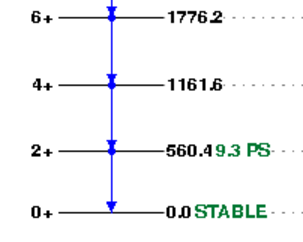
\includegraphics{images/te_120_rot}
    \caption{Rotational structure in Te-120. Notice that the $2^+$,
      $4^+$, and $6^+$ states are all evenly spaced.}
    \label{fig:te120}
  \end{figure}
\end{itemize}

\subsection{Independent Particle Model}
\begin{itemize}
\item All shells are completely full or empty except for a single
  particle in the lowest energy of an otherwise empty shell. The
  nucleus $J^\pi$ depends only on that last
  nucleon. \cite[Lec. 13-16]{lecture}.
\item The total angular momentum of the nuclei $J$ is equal to the
  $J$ value of the shell with the single particle in it. The parity
  is equal to the parity of the shell with the single particle in it,
  $(-1)^l$. For example, if there is a single particle in the
  $1p_{3/2}$ state, then $J^\pi=(\frac{3}{2})^{-}$ because
  $j=\frac{3}{2}$ and $l=1$. \cite[Lec. 13-16]{lecture}.
\item The value $J^\pi$ is referred to as the spin-parity \textbf{or}
  the total angular momentum of the nucleus. Both of those
  things mean the same thing \textit{when you're talking about the
    nucleus.} For a nucleon, spin is the intrinsic angular momentum;
  the nucleus doesn't have any \textbf{intrinsic} angular momentum,
  only angular momentum due to it's components. We call it spin anyway
  when referring to the nucleus just to be confusing.
\item The independent nucleon always gives the total angular momentum
  of the shell to the nucleus when in the \textbf{ground state.}
\item When you are in an \textbf{excited state}, you can line up the
  nucleons in more interesting way. If you have three nucleons in the
  $f_{7/2}$ shell and we're in an excited state, we use the notation
  $(f_{7/2)})^3$. You can add up their angular momentum any way you
  want, remember each can have angular momentum from $-j$ to $+j$. So
  these can have $m=\pm\frac{1}{2}, \pm\frac{3}{2}, \pm\frac{5}{2},
  \pm\frac{7}{2}$. They can't have the \textbf{same} value of m, but
  they can all add to get, for example
  $\frac{7}{2}+\frac{5}{2}+\frac{3}{2}=\frac{15}{2}$.~\cite[pp. 149-151]{krane}
\item In excited states, the single nucleons can also jump around to
  other states, changing the $J^\pi$ of the nucleus.~\cite[Lec. 13-16]{lecture}
\end{itemize}

\section{Collective Motion}

\begin{itemize}
\item Collective nuclear motion comes from the interplay between
  nucleons making the nuclear potential, and nucleons moving in the
  nuclear potential.~\cite[Lec. 13-16]{lecture}
\item Collective motion lowers the energy for the first excited state
  ($2^+$ for vibration and rotation). Instead of having to yank
  a nucleon from a low, tightly bound state, to a high state, you just
  put enough energy into the system to get all the nucleons vibrating
  or rotating together. So nuclei where collective motion is seen have
  much, much lower first excited states.
\item Rotations and vibrations and not mutually
  exclusive. A rotational band can ``ride'' on top of a vibration, or
  vice versa.
\item The collective model is useful and good when there are a large
  number of valence nucleons, promiscuity:
  \begin{equation*}
    P=\frac{N_pN_n}{N_p+N_n}
  \end{equation*}
Where $N_p$ is the number of valence protons, and $N_n$ is the number
of valence neutrons. Valence nucleons are the extra nucleons after the
last large shell. Around 4, you see collective motion.~\cite[Lec. 13-16]{lecture}
\end{itemize}

\subsection{Vibration}
\begin{itemize}
\item A vibration can move over the surface of the nucleus. The order
  of this vibration is given by lambda ($\lambda$), this determines
  the order of the spherical harmonic that describes the collective vibration.
  \begin{itemize}
  \item The $\lambda=1$ vibration is just dipole movement, which
    is just linear movement of the nucleus. This is not a collective
    motion state.
  \item The $\lambda=2$ vibration is the quadrupole vibration. The
    energy is quantized in the \textit{phonon} which is just a
    discrete unit of vibrational energy. For $\lambda=2$, each carries
    exactly $2\hbar\omega$ units of vibrational energy.
  \item The $\lambda=3$ vibration is octopole and I'm pretty sure Lee
    said this hasn't been observed.
  \end{itemize}
\cite[Lec 13-16]{lecture}
\item A vibration collective structure on top of the $0^+$ ground
  state will be a $2^+$ level, followed by a $4^+$ level, followed by
  $6^+$, etc.  They will be
  \textit{evenly spaced} in energy, because each level represents the
  addition of one phonon and each phonon has the same energy. The
  parity doesn't change because $\lambda=2$ and parity goes like
  $(-1)^\lambda$.~\cite[Lec 13-16]{lecture}
\item Therefore, he ratio of the $4^+$ and $2^+$ states should almost always be:
  \begin{equation*}
    R_{42}=\frac{E(4^+)}{E(2^+)} \approx 2
  \end{equation*}

\end{itemize}

\subsection{Rotation}
\begin{itemize}
\item There is an enhanced probability of decay between rotational
  bands because the wave functions are all the same, or very similar.
%R42=3.3
\item The ratio of the $4^+$ and $2^+$ states should almost always be:
  \begin{equation*}
    R_{42}=\frac{E(4^+)}{E(2^+)} \approx 3.3
  \end{equation*}

\end{itemize}


\section{$\alpha$-decay}

\begin{itemize}
\item The $\alpha$-decay half-life can be estimated using a barrier
  tunneling model. You can calculate the frequency of collision with
  the potential well and use the transmission probability to calculate
  a half-life. This isn't the real model and only represents an
  electromagnetic baseline to give us insight into what is
  happening. It isn't \textit{nuclear}.~\cite[Lec. 18]{lecture}
\item Any angular momentum carried away by the $\alpha$-particle is
  \textbf{purely orbital}. The spins all couple pairwise to
  0. The angular momentum change from $\alpha$-decay can range from:
  \begin{equation*}
    |I_i-I_f| \leq l_{\alpha} \leq I_i + I_f
  \end{equation*}
With parity change:
\begin{equation*}
  \Delta\pi = {(-1)}^{l_{\alpha}}
\end{equation*}
The simplest decay is any $0 \to X$ state, because the only value
for $l_{\alpha}$ is $X$. If that doesn't give the right parity change,
the decay is \textit{forbidden}. In this case it really means
\textit{forbidden}, unlike $\beta$-decay, which plays fast and loose
with the term.~\cite[pp. 257-258]{krane}.
\item $\alpha$-decay can populate many different states. Each one has
  a different $Q$-value (given by the $Q$ value for decay to the
  ground state, minus the excitation
  energy).~\cite[pp. 257-258]{krane}.
\item The intensity depends on how similar the initial and final wave
  functions are, and the angular momentum ($l_{\alpha}$).~\cite[pp. 257-258]{krane}.
\item The hinderence factor (HF) tells us about the similarity between
  the parent and daughter states.:
  \begin{itemize}
  \item $1<H<4$ Favored: $\alpha$-particle is from two low-lying pairs
    of nucleons.
  \item $4<H<10$: favorable overlap between initial and final state.
  \item $10<H<100$: spin projections are parallel. Unfavorable overlap
    between initial and final states.
  \item $100<H<1000$: spin projections are parallel, change in parity.
  \item $H>1000$: spin-flip, change in parity.
  \end{itemize}
Any spin flip $\to$ over 1000. Any parity change $\to$ over
100. Non-favorable overlap $\to$ over 10. See
Table.~\ref{tab:alpha-hinderance}.~\cite[Lec. 18]{lecture}
\begin{table}[hbt]
\centering
\begin{tabular}{llll}
\textbf{H}       & \textbf{Nuclear State Overlap} & \textbf{Parity Change} & \textbf{Spins} \\
\textless10   & Favorable                      & None                   & Parallel       \\
10--100           & Unfavorable                    & None                   & Parallel       \\
100--1000         & Unfavorable                    & Yes                    & Parallel       \\
\textgreater1000 & Unfavorable                    & Yes                    & Spin-flip      \\
                 &                                &                        &               
\end{tabular}
\caption{Summary of $\alpha$-decay hinderance factors.}
\label{tab:alpha-hinderance}
\end{table}
\item $\alpha$-decay spectrum has sharp peaks, each represents a decay
  to different excited states. Higher $E_\alpha$, lower excitation
  energy. The excited states then usually release $\gamma$-ray
  photons.~\cite[pp. 262-264]{krane}
\item In an even-even nucleus, the alpha decay to the ground state is
  usually \textit{very strong}. The $0^+ \to 0^+$ decay is not
  inhibited by differences between the wave functions (they are very
  similar. By the same logic, the decay of odd-$A$ nuclei may be
  \textit{very weak} because the two states may be significantly
  different.~\cite[pp.264]{krane}
\end{itemize}

\section{$\beta$-decay}
\begin{itemize}
\item Energy release distribution is continuous because there are two
  particles emitted so they can share any proportion of the
  energy.~\cite[pp. 273, Lec 19]{krane,lecture}
\item Three kinds:
  \begin{equation*}
    \begin{split}
    \beta^-&: n \to p + e^- + \bar{\nu}_e \\
    \beta^+&: p \to n + e^+ + \nu_e \\
    EC&: p + e^- \to n + \nu_e
  \end{split}
  \end{equation*}
Each has a different energy release:
\begin{equation*}
  \begin{split}
    Q_{\beta^-}&=[m(^AX)-m(^AX')]c^2 \\
    Q_{\beta^+}&=[m(^AX)-m(^AX')-2m_e]c^2\\
    Q_{\epsilon}&=[m(^AX)-m(^AX')]c^2-B_n
  \end{split}
\end{equation*}
For $\beta^-$, the electron masses all cancel when using atomic masses
because $-Zm_e+(Z+1)m_e-m_e=0$, that is the electrons accounted for in
the atomic masses for the original atom, final atom and leftover
electron all cancel. They don't cancel for $\beta^+$ because
$-Zm_e+(Z-1)m_e-m_e=-2m_e$.~\cite[pp. 274-276]{krane}

\subsection{Fermi Theory}

\item There are three things that go into
  determining the spectrum of beta decay energy values:
  \begin{equation*}
    \begin{split}
    N(p) &\propto \text{Statistical factor} * \text{Coulomb Interaction
    (electrodynamic)} * \text{Nuclear Matrix Element} \\
  N(p) &\propto p^2(Q_\beta-T_e)^2*F(Z_d,T_e)*|M_{fi}|^2*S(p,q)
\end{split}
\end{equation*}
These terms are:
\begin{itemize}
\item Statistical factor: related to the number of final states
  accessible. Decays like to happen when there are a lot of final
  states that are open.
\item Fermi function ($F$): the influence of the atomic coulomb
  field. This is the \textbf{electrodynamic} part.
\item Matrix element ($M_{fi}^2*S(p,q)$): This is the \textbf{Nuclear}
  part. It is kind of like the hinderance factors for $\alpha$-decay
  and represents the effect of the initial and final states. The $S$
  function only comes into play in \textbf{forbidden} decays, when the
  electron and neutrino have angular momentum ($l \neq 0$, $s$ and $q$
  are terms for the electron and neutrino angular momenta.
\end{itemize}
\cite[pp.281-282]{krane}.
\item You can plot:
  \begin{equation*}
    (Q-T_e) \propto \sqrt{\frac{N(p)}{p^2F(Z',p)}}
  \end{equation*}
Which \textit{should} give you a straight line (Fermi-Kurie plot) that intersects the
$x$-axis at the $Q$ value. For forbidden decays, the line is
\textbf{not} straight, you have to put that $S(p,q)$ factor in on the
bottom to make it straight. This is the \textit{shape factor}, which
then gives you a straight line.~\cite[pp. 282]{krane}
\item Total decay rate: you can integrate some messy function to get a
  messy function for total decay rate:
  \begin{equation*}
    \lambda = \text{Matrix Element Term} * \int\text{$F$-function and statistical factor}
  \end{equation*}
The full equation is in Krane, page 282. What is important is that the
term outside the $\int$ is the \textbf{nuclear} part, and the integral
is the \textbf{electrodynamic} part. Those are the two things (and
some constants) that determine the decay rate. You can just crunch the
integral and look up values, which is $f$, or the \textit{Fermi
  Integral}. Then, if you do $\frac{f}{\lambda}$ or just $ft_{1/2}$,
then the integrals cancel and all you have is the Matrix Element part,
the \textbf{nuclear} part. This lets us compare $ft_{1/2}$ values,
which are \textit{only dependent on nuclear
  properties}. It might be useful to think about the $ft$ value as just a
\textit{corrected} half-life. Corrected to remove electrodynamic stuff.~\cite[pp. 282-283, Lecs. 19-21]{krane,lecture}.
\item $ft$ values have a huge range ($10^3$ to $10^{20}$) so we use
  log$ft$ instead.
\end{itemize}
\subsection{Allowed Decays}

\begin{itemize}
\item Electron and neutrino are created at the origin ($r=0$), so
  their angular momentum is $l=0$. There are two modes based on spin:
  \begin{itemize}
  \item \textbf{Fermi Decay}: the spins of the neutrino and electron
    are anti-parallel, so total $S=0$.
  \item \textbf{Gamow-Teller Decay:} the spins are parallel, so the
    total $S=1$.
  \end{itemize}
The difference in the nuclear spin parity ($I^\pi$) before and after
the decay will come from the
$l$ and $S$ that the electron and neutrino carry away. So, if you have
Fermi decay ($l=0$ and $S=0$), there can't be any change in the
nuclear spin $\Delta{}I = |I_i-I_t|=0$. If you have Gamow-Teller decay
($l=0$ and $S=1$), you have $\Delta{}I =$ 0 or 1. 
\begin{framed}
  \textbf{TRICKY PART:} You can have $\Delta{}I = 0$ in Gamow-Teller decay because you can
  couple a vector of length 1 onto a vector and end up with the same
  vector magnitude. This \textbf{does not work} if you started with
  $I_i=0$ because you can't add 1 to 0 and get 0. This means that a
  beta decay from $I_i=0$ to $I_f=0$ \textit{must} be Fermi decay.
\end{framed}
Therefore, all allowed decays have:
\begin{equation*}
  \Delta{}I = 0,1 \quad \Delta{}\pi = \text{no}
\end{equation*}
\cite[pp. 289, Lec. 19-21]{krane,lecture}
\item \textbf{Superallowed Decays:} all super-allowed decays are
  allowed decays, but not all allowed decays are super-allowed. All
  that super-allowed means is that the $ft$ value is 3-4. So they are
  just super-likely.
\end{itemize}

\subsection{Forbidden Decays}

\begin{itemize}
\item Any beta-decay that has $l \neq 0$ is \textbf{forbidden}. This
  doesn't mean that it doesn't happen, it just means it's not very
  likely. This is because angular momentum $\vec{l} =
  \vec{r}\bullet\vec{p}$. The radius where the $\beta$-decay is on the
  order of the nuclear radius ($\approx$ 6 fm) which is \textit{super}
  small. The small radius means a small angular momentum, so it's very
  unlikely that $\beta$-decay will occur with $l \neq 0$. But it does,
  rarely.~\cite[Lec. 19-21]{lecture}.
\item The n\textsuperscript{th} forbidden decay will have $l=n$, and both of the
  spin-arrangements (Fermi for $S=0$ and Gamow-Teller for $S=1$)
  described above. Therefore, you can have:
  \begin{equation*}
    \Delta{}I=0,1,2\ldots(n+1) \quad \Delta\pi = (-1)^n
  \end{equation*}
The $\Delta{}I$ goes up to $n+1$ because Gamow-Teller can have the
spin $S=1$ lined up with the angular
momentum.~\cite[pp.291,Lec.19-21]{krane,lecture}
\item $\beta$-decay will occur via the ``lowest'' decay that it
  can. That is, it will use an allowed decay or the lowest nth
  forbidden decay that can accomplish the transition. You have to look
  at \textit{both} parts of the initial and final states, $I$
  \textbf{AND} $\Delta\pi$ to figure out which it is.~\cite[Lec 19-21]{lecture}
\item Based on the description above, as you get higher in the
  forbidden decays, 1st forbidden to 2nd forbidden etc, the decays
  become less likely. See Table~\ref{tab:logft}.~\cite[Lec. 19-21]{lecture}
\begin{table}[hbt]
\centering
\begin{tabular}{lr}
\textbf{Type of $\beta$-decay} & \textbf{Log($ft$)} \\
Superallowed                   & 3.5                \\
Allowed                        & 4-7.5              \\
1st forbidden                  & 6-9                \\
2nd forbidden                  & 10-13              \\
3rd forbidden                  & 14-20              \\
4th forbidden                  & $\approx$ 23      
\end{tabular}
\caption{Log($ft$) values for types of $\beta$-decay}
\label{tab:logft}
\end{table}
\end{itemize}

\subsection{Electron Capture}

\begin{itemize}
\item Almost always, the electron is captured from the inner-most $S$
  orbital, and the neutrino emitted is mono-energetic. Auger electrons
  may result from the cascade of electrons as they move down to fill
  the vacancy left by the lower shells.~\cite[Lec. 19-21]{lecture}
\end{itemize}

\subsection{Helicity}

\begin{itemize}
\item Helicity: helicity is just a property that we define based
  on a particles spin and momentum:
  \begin{equation*}
    h=\frac{\vec{s}\bullet\vec{p}}{|\vec{s}\bullet\vec{p}|}
  \end{equation*}
  Neutrinos have specific helicity based on if they are a neutrino or
  anti-neutrino:
  \begin{itemize}
  \item \textbf{ALL} neutrinos ($\nu$) have helicity $h=-1$
  \item \textbf{ALL} anti-neutrinos ($\bar{\nu}$) have helicity $h=+1$
  \item All electrons \textbf{from $\beta$-decay} have helicity
    $h=-\frac{v}{c}$.
  \item All positrons \textbf{from $\beta$-decay} have helicity
    $h=+\frac{v}{c}$.
  \end{itemize}
  Note that the helicity rules for neutrinos are always always true,
  but the ones for electrons/positrons are only true \textit{if the
    electron is from $\beta$-decay}.
\end{itemize}

\section{$\gamma$-decay}

\begin{itemize}
\item $\gamma$-rays are photons generated from the decay between two
  nuclear states.
\end{itemize}

\bibliographystyle{unsrt}
\bibliography{NE101}
\end{document}
